\documentclass[12pt,fleqn]{article}\usepackage{../../common}
\begin{document}
Makro Bilgisi ve Piyasaların Gidişatının Bağlantısı

Hedgeye kuruluşunun CEO'su Keith Mccollough (KM) başlangıç olarak iki değişkene
bakarak genel olarak hangi varlıklara, ne zaman yatırım yapılması gerektiğine
karar verebilmekte. Bu iki değişken enflasyon ve ekonomik büyümedir. Fakat
önemli bir nokta KM bu değişkenlerin ikinci türevine bakıyor, yani değişimin
değişimine, ya da değişim hızına (rate of change). Fizikle alakalandırmak
gerekirse enflasyonun ``ivmesinden'' ya da ``frenlemesinden (ters ivme)''
bahsediyor mesela ki ivme ikinci türevdir (mesafenin zamana göre türevi hız,
onun türevi ivme). Niye ikinci türev? Çünkü KM tarihi veriye bakarak bulmuştur
ki enflasyon ve büyümenin değişim hızı senetlerin, o dönemdeki tahvillerin,
senetlerin getirisi ile çok yakından bağlantılıdır.

Değişimin değişimini KM şu şekilde hesaplıyor: ilk türev yıl-üzeri-yıl
(year-over-year, YoY) üzerinden yani, mesela, bir çeyrek için büyüme yüzdesi
hesaplanacaksa bu aynı senedeki bir önceki çeyreğe değil, 1 sene önceki aynı
çeyreğe bakılarak yapılıyor. Böylece elmaları elmalar ile karşılaştırmış oluruz,
mevsimsel farklılıklar hakkında endiselenmek gerekmez. Eğer 2010 senesindeki
4. çeyrek, 3. çeyrekten büyük ise, belki bu büyüklük kış sezonunda bazı
eylemlerin hep daha fazla olmasindan ileri geliyordur, yani büyüme ``gerçek''
değil sezonsaldır. Ama 2010 4. çeyreği 2009 4. çeyreği ile karşılaştırırsak bu
mevsimsel farklılıkları hesaba almamış oluruz. Bu birinci türev. Bu zaman serisi
hesaplandıktan sonra ikinci ikinci fark / türev hesabı bir önceki öğeye bakarak
klasik şekilde yapılabilir.

Enflasyon aynı şekilde, YoY, sonra klasik fark.

Genel olarak düşünmek gerekirse KM makro değişkenlerini, ekonomiyi çevrimsel /
dönemsel (cycliç) olarak görüyor, aynen bir yılın mevsimleri olduğu gibi. İnen
bir süre sonra aşağı inmek zorundadır, düşen bir süre sonra yukarı çıkmak
zorundadır. Bu bir çember görüntüsü kafamızda oluşturabilir, ya da zaman
indisini de hesaba katarsak sağa doğru açılmış bir çember, yani bir sinüs
eğrisinden bahsediyoruz. Her değişken KM'e göre bir sinüs eğrisinde hareket
etmektedir; enflasyon ve büyüme sinüs eğrilerinin de tabii kendine has
parametreleri olabilir, bazıları daha geniştir belki bazıları daha dardır,
genliği kimisinin daha yüksektir. Farklı ülkelerin büyümeleri de farklı
eğrilerde olacaktır. Ama KM tüm değişkenleri sinüste farzeder. O zaman metodun
yaptığı bir değişkenin ikinci türevine bakarak sinüs eğrisinin neresinde
olduğunu anlamaya uğraşmaktır. Bu anlayışın getirdiği ilk rapor altta.

ABD verisi üzerinde uygulayalım,

\begin{minted}[fontsize=\footnotesize]{python}
import pandas as pd

df1 = pd.read_csv('quandl-gdp.csv',index_col=0,parse_dates=True)
df2 = pd.read_csv('quandl-inf.csv',index_col=0,parse_dates=True)

df1['gdpyoy'] = (df1.Value - df1.Value.shift(4)) / df1.Value.shift(4) * 100.0
def f(x):
    if x.name.month == 4: return "%d%s" % (x.name.year,"Q1")
    elif x.name.month == 7: return "%d%s" % (x.name.year, "Q2")
    elif x.name.month == 10: return "%d%s" % (x.name.year, "Q3")
    elif x.name.month == 1: return "%d%s" % (x.name.year-1, "Q4")

df1['Q'] = df1.apply(f, axis=1)
print (df1[['gdpyoy','Q']].tail(3))

df2['cpi'] = df2.resample('Q')[['Value']].mean()
df2c = df2.dropna()

def f(x):
    if x.name.month == 3: return "%d%s" % (x.name.year,"Q1")
    elif x.name.month == 6: return "%d%s" % (x.name.year, "Q2")
    elif x.name.month == 9: return "%d%s" % (x.name.year, "Q3")
    elif x.name.month == 12: return "%d%s" % (x.name.year, "Q4")

df2c['Q'] = df2c.apply(f, axis=1)
print (df2c[['cpi','Q']].tail(3))
print (df2c.tail(3))
\end{minted}

\begin{verbatim}
              gdpyoy       Q
Date                        
2018-01-01  2.580414  2017Q4
2018-04-01  2.869807  2018Q1
2018-07-01  3.039632  2018Q2
                 cpi       Q
Date                        
2018-03-31  2.214333  2018Q1
2018-06-30  2.712000  2018Q2
2018-09-30  2.642000  2018Q3
            Value   ...         Q
Date                ...          
2018-03-31  2.360   ...    2018Q1
2018-06-30  2.872   ...    2018Q2
2018-09-30  2.277   ...    2018Q3

[3 rows x 3 columns]
\end{verbatim}

\begin{minted}[fontsize=\footnotesize]{python}
df = df1[['gdpyoy','Q']].merge(df2c[['cpi','Q']], on='Q')
df['gdpyoy'] = df.gdpyoy.shift(1)
df['gdpdiff'] = df.gdpyoy.diff()
df['cpidiff'] = df.cpi.diff()
df = df.dropna()
\end{minted}

Değişim hızını üstteki şekilde elde edince şimdi çok önemli bir raporu ortaya
çıkarmak mümkün. İki değişken +, -, yani ivmeleneme, frenleme üzerinden 4 farklı
şekilde kombine edilebilir; hem büyümede hem enflasyonda ivme vardır, ya da
büyümede ivme enflasyonda fren vardır, vs. bu dört kombinasyonu Quad (Bölge) 1,
Quad 2, Quad 3, .. diye ayrılır. KM her quad'ın kendine has özellikleri, yatırım
usulleri olduğunu söyler (çünkü geçmise dönük analizi ona bu fikri vermiştir).

\begin{minted}[fontsize=\footnotesize]{python}
import random
plt.xlim(-1.0,1.0)
plt.ylim(-1.0,1.0)
plt.grid()
res = df[['Q','cpidiff','gdpdiff']].tail(14)
for (q,x,y) in np.array(res):
    plt.plot(x,y,'rd')
    xa = random.choice(np.linspace(0,0.05,3))
    plt.text(x+xa,y+xa,q)
plt.savefig('tser_macromkt_03.png')    
\end{minted}

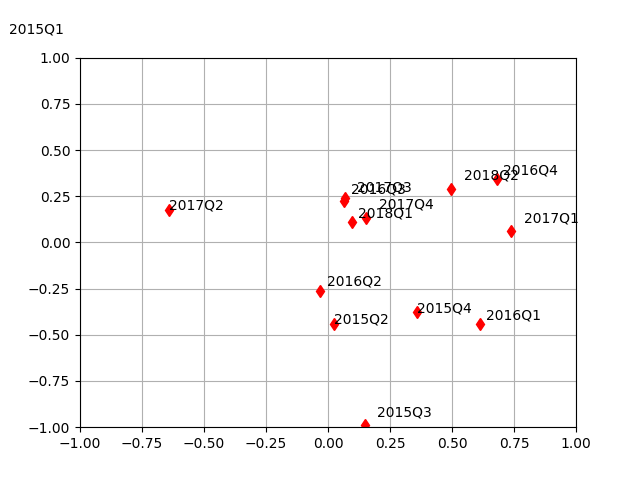
\includegraphics[width=20em]{tser_macromkt_03.png}

Geçmişe dönük Quad'ların nerede olduğunu görüyoruz. Quad 1 iyi, Quad 2 çok
iyi. Her iki durumda da büyüme yukarı çıkıyor. Quad 2'de büyüme ve enflasyon
aynı anda yukarı çıkıyor. Bu bölgede herşey kazanıyor, tek istisnalar altın,
tahviller ve dolar. Kıyasla Quad 4'te büyüme ve enflasyon aynı anda aşağı
iniyor, burada dolar, aşağı beta defansif hisseler, günlük ihtiyaçlara hitap
eden şirketler (enerji, alışveriş, vs), tahviller. Satılacaklar momentum,
büyüme, ve Google, Microsoft gibi teknoloji şirketleri.

Not: Beta bir senetin tüm borsaya nazaran oynaklığıyla alakalı, borsadaki tüm
senetler üzerinden hesaplanan oynaklık sayısı 1 kabul edilir, bunun altında (kat
bağlamında) olan her diğer senet oynaklığı bu beta biriminden raporlanır. Mesela
bir senetin oynaklığı borsa oynaklığının iki katıysa ona ``2 beta'' senedi
denir, yarısıysa ``0.5 beta''.

Quad 3 stagflasyon. Bu noktaya çoğunlukla Quad 4'te olduğunu farkeden merkez
bankaları yüzünden gelinir. Merkez bankacı panikleyerek kuru devalue eder,
değerini indirir, ve ``varlık fiyatı enflasyonu'' yaratırlar, senetlerde, emlak
piyasasında mesela. Çinliler bunu 2018'de yaptılar, Quad 4'teydiler, yuan'ı
yüzde 4 devalüe ettiler, ve varlıklarda enflasyon pompalayarak ``büyüme hayali''
yarattılar, ama sonucunda ekonomik stagflasyona mahkum oldular.

Quad 2 ile Quad 4 birbirinin neredeyse tam zıttı. Birinde iyi olan diğerinde
kötü, ve diğer şekilde.

Enflasyon ve büyüme bu kadar önemli kararları etkilediği için onları tahmin
edebilen makro geleceği tahmin eder, ve Hedgeye şirketi bu ise müthiş
odaklıdır. Aslında kabaca düşününce bu tahminin imkansız olmayacağı anlaşılır,
eğer sinüs eğrisinin neresinde olacağımızı tahmin etmeye uğraşıyorsak, bunu
nerede olduğumüza, nereden geldiğimize bakarak yapabilmemiz gerekir. HE
hakikaten YoY verisinden geriye bakarak ortalamaya dönüş zamanını, işaret
değişimini tahmin edebiliyor. Tam değişim hızı tahmini için 30 tane makro
faktörü kullanarak bir başka regresyon yapıyorlar [10].

İma Edilen Oynaklık (İmplied Volatility)

HE sistemi Quad'lara ek olarak gerçek / tarihi ve ima edilen oynaklık [5,6,7]
arasındaki ilişkiye bakarak ta işlem yapıyor. İma edilen oynaklık gelecekteki
oynaklıktır. Fakat gelecekteki oynaklığı nasıl tahmin edeceğiz?

Belki başkalarının yaptığı tahmini kullanarak kendi tahminimizi
oluştururuz. Ekler bölümünde opsiyonları anlattık; $\sigma$ tahmininin
Black-Scholes formülüne dışarıdan verilerek opsiyon fiyatlaması yapıldığını
biliyoruz. Biz bu sistematiği tersine çevirerek başkalarının hesapladığı /
verdiği / yayınladığı opsiyon fiyatlarından geriye giderek ima edilen oynaklığı
elde edecegiz.

B-S formülünün kendisinin türetilmesine burada girmeyeceğiz, onu sadece şu
şekilde gösterelim,

$$
V = BS(S,K,r,T,\sigma)
$$

ki $S$ o andaki senet fiyatı, $K$ kullanım (strike) fıyatı, $r$ risksiz faiz
oranı, $T$ ise opsiyonun bitişine kadar geçecek zaman. Dikkat edersek $\sigma$
haricindeki tüm parametreler biliniyor.

Bir örnek üzerinde görelim, piyasada mevcut opsiyonlara baktığımızda GOOG
(Google) için 18 Ekim 2014'te biten bir opsiyon görüyoruz, kullanım fiyatı
\$585, teklif fiyatı \$17.50. Yani $V,K,T$ elimizde. Bugünkü (opsiyon bitişinden
kabaca bir ay önce, 9 Eylül) senet fiyatlarına bakıyoruz, GOOG \$586.08
seviyesinde, bu da $S$. Risksiz faiz $r$ için 4 haftalık tahvil faizlerine
bakabiliriz, ki o da şu anda \%0.02 seviyesinde. Bu verilerle

$$ V = BS(S,K,r,T,\sigma) $$

$$ 17.50 = BS(586.08, 585.00, 0.0002, 0.10958.., \sigma)$$

Şimdi elimizde tek bilinmeyen $\sigma$. Fiyatlandırmayı yapan kuruluşlar tabii
ki oraya bir değer girerek 17.50 fiyatını bulmuşlar, biz $\sigma$ harici bilinen
tüm parametreleri kullanıp tek bilinmeyen $\sigma$'yi bulmaya uğraşacağız [8].

Ne yazık ki B-S denklemini cebirsel olarak tekrar düzenleyip $\sigma$'yı
eşitliğin bir tarafında tek başına bırakmak analitik olarak mümkün
değil. Ama sayısal kök bulma yöntemlerini kullanabiliriz. Bu yöntemlerden
Newton'un yöntemini [11] yazısında gördük. Bir $f(x)$ için $f(x)=0$
sonucunu verecek $x$ değerlerini bulmak kök bulmaktır. Tabii üstteki
problemde sıfıra değil, belli bir sabit değere olan eşitlik var, $f(x) = a$
gibi, ama bu önemli değil, bu problemi sıfıra eşitliği baz alan kök bulmaya
çevirebiliriz, $g(x) = a-f(x) = 0$ ile mesela. Ardından Newton yöntemini
yine olduğu gibi, $g$ üzerinde kullanırız,

$$
x_{n+1} = x_n - \frac{g(x_n)}{g'(x_n)}
$$

ya da 

$$
x_{n+1} = x_n - \frac{a-f(x_n)}{f'(x_n)}
$$

Peki türev $g'(x)$ nereden geliyor? B-S türetimini bilenler oynaklığa göre
$g(x)$'nin türevinin ``vega fonksiyonu'' olduğunu bilirler. Bu fonksiyon B-S
matematiği içinde bilinen, standart bir fonksiyon.

\begin{minted}[fontsize=\footnotesize]{python}
from scipy.stats import norm
import datetime, numpy as np

def find_vol(target_value, call_put, S, K, T, r):
    MAX_ITERATIONS = 100
    PRECISION = 1.0e-5

    sigma = 0.5
    for i in range(0, MAX_ITERATIONS):
        price = bs_price(call_put, S, K, T, r, sigma)
        vega = bs_vega(call_put, S, K, T, r, sigma)
        diff = target_value - price  # our root

        print (i, sigma, diff)

        if (abs(diff) < PRECISION): return sigma
        sigma = sigma + diff/vega # f(x) / f'(x)

    return sigma


n = norm.pdf
N = norm.cdf

def bs_price(cp_flag,S,K,T,r,v,q=0.0):
    d1 = (np.log(S/K)+(r+v*v/2.)*T)/(v*np.sqrt(T))
    d2 = d1-v*np.sqrt(T)
    if cp_flag == 'c':
        price = S*np.exp(-q*T)*N(d1)-K*np.exp(-r*T)*N(d2)
    else:
        price = K*np.exp(-r*T)*N(-d2)-S*np.exp(-q*T)*N(-d1)
    return price

def bs_vega(cp_flag,S,K,T,r,v,q=0.0):
    d1 = (np.log(S/K)+(r+v*v/2.)*T)/(v*np.sqrt(T))
    return S * np.sqrt(T)*n(d1)

def test1():
    
    V_market = 17.5
    K = 585
    T = (datetime.date(2014,10,18) - datetime.date(2014,9,8)).days / 365.
    S = 586.08
    r = 0.0002
    cp = 'c' # call option
    
    implied_vol = find_vol(V_market, cp, S, K, T, r)
    
    print ('Ima edilen oynaklik (implied vol): %.2f%%' % (implied_vol * 100))
    
    print ('Piyasa fiyat (market price) = %.2f' % V_market)
    print ('Model fiyati (model price) = %.2f' % bs_price(cp, S, K, T, r, implied_vol))

test1()
\end{minted}

\begin{verbatim}
0 0.5 -21.669539271534063
1 0.21879739316064523 0.03217154881230044
2 0.21921383628613422 1.9891615465894574e-08
Ima edilen oynaklik (implied vol): 21.92%
Piyasa fiyat (market price) = 17.50
Model fiyati (model price) = 17.50
\end{verbatim}

Bir sonuç bulduk. Şimdi opsiyona baktığımızdaki gerçek oynaklık ile bir ay
sonrasındaki gerçek oynaklığı karşılaştıralım. Acaba ima edilen oynaklığın
geleceği tahmin edici kuvveti var mı?

\begin{minted}[fontsize=\footnotesize]{python}
import pandas as pd
df = pd.read_csv('GOOG.csv')
print (len(df))
print ('8 eyluldeki gercek oynaklik', np.std(df['Close'].head(252).pct_change()) * np.sqrt(252))
print ('18 ekimdeki gercek oynaklik', np.std(df['Close'].tail(252).pct_change()) * np.sqrt(252))
\end{minted}

\begin{verbatim}
281
8 eyluldeki gercek oynaklik 0.24023589641421986
18 ekimdeki gercek oynaklik 0.20560500728697875
\end{verbatim}

Yüzde 24'ten yüzde 20'ye bir iniş var, ve üstteki hesaptan da tahmin olarak
yüzde 22 elde ettik, yani orada da bir iniş tahmin edildi. 

Not:

Altta daha önce Yahoo finans servisinen indirilmiş opsiyon verisi üzerinde bazı
işlemleri görüyoruz. Bunları referans amaçlı burada tutuyoruz. Dikkat edersek
veride `İV` adında bir kolon var, bu kolon ima edilen oynaklık olarak
gösterilir. Ne kadar gerçeği yansıtıyor bilmiyoruz, ama aklımızda olsun, bu
kolonu da belki olduğu gibi kullanmak mümkündür. 

\begin{minted}[fontsize=\footnotesize]{python}
import pandas as pd
import numpy as np
from datetime import datetime
from datetime import date
import pandas_datareader.data as web

pd.set_option('display.notebook_repr_html', False)
pd.set_option('display.max_columns', 7)
pd.set_option('display.max_rows', 10) 
pd.set_option('display.width', 82) 
pd.set_option('precision', 3)
\end{minted}

\begin{minted}[fontsize=\footnotesize]{python}
aapl_options = pd.read_csv('aapl_options.csv',  parse_dates=['Expiry'])
aapl_options['IV'].tail(4)

aos = aapl_options.sort_values(['Expiry', 'Strike'])[['Expiry', 'Strike', 'Type', 'IV', 'Bid', 'Ask', 'Underlying_Price']] 
aos['IV'] = aos['IV'].apply(lambda x: float(x.strip('%')))
aos[:5]

aos['Expiry'].unique()

aos.loc[158]

calls1 = aos[(aos.Expiry=='2015-02-27') & (aos.Type=='call')]
calls1[:5]
\end{minted}

\begin{verbatim}
Out[1]: 
        Expiry  Strike  Type      IV    Bid    Ask  Underlying_Price
158 2015-02-27    75.0  call  271.88  53.60  53.85            128.79
190 2015-02-27    80.0  call  225.78  48.65  48.80            128.79
226 2015-02-27    85.0  call  199.22  43.65  43.80            128.79
265 2015-02-27    90.0  call  175.00  38.65  38.80            128.79
303 2015-02-27    93.0  call  160.16  35.65  35.80            128.79
\end{verbatim}

Kaynaklar

[1] Hedgeye, Ana Ders, \url{www.youtube.com/watch?v=hS-JOXZrcdU}

[2] Hedgeye, Ana Ders, \url{www.youtube.com/watch?v=2NvNGAIvcb0}

[3] Hedgeye, Ana Ders, \url{youtu.be/V-uoyDj0tKs}

[4] Hedgeye, Ana Ders, \url{youtu.be/27SQ5mYf38k}

[5] Hedgeye, Oynaklik, \url{youtube.com/watch?v=FwpckOfUyRk}

[6] Hedgeye, Oynaklik, \url{youtube.com/watch?v=-WJtepxbQbE}

[7] Hedgeye, Oynaklik, \url{youtube.com/watch?v=USrojq9tgzs}

[8] Codeandfinance, {\em Finding implied volatility},
    \url{http://www.codeandfinance.com/finding-implied-vol.html}

[9] Heydt, {\em Mastering Pandas for Finance}

[10] Hedgeye, \url{http://app.hedgeye.com/mu/he_2q18_macrothemes_update_5-4-2018?encoded_data=ftvm,3MW2y7jAWWk/RR9BK6C07dDZp9A=,}

[11] Bayramli, Diferansiyel Denklemler, {\em Kök Bulmak, Karesel Formül}

\end{document}

